\section{Results}
This section contains the results obtained during the design process of the whole the project.
\subsection{Discharge Flow Control Unit}
\subsubsection{Flow control sub-unit}
An MG996R servo motor was selected for this sub-unit, to open and close the valve in steps that can be less than $1^{0}$ depending on the number of steps requested by the user. Direct pulse width modulation was preferred to a micro-step drive as a mechanism to drive the servo motor in steps of any size.
\par
A mounting mechanism for the servo motor was designed to the specifications of the motor and finite element analysis conducted as shown in figure \ref{fig:servo_assembly_results} .   
\begin{figure}[H]
      \centering
         \includegraphics[width=\textwidth]{Figures/ServoHolderBallValveAssembly-Static-1-1-1.png}
          \caption{Servo Assembly simulation results}
          \label{fig:servo_assembly_results}
      \end{figure}
    The interface and the servo mounting rods were subjected to stress analysis. With the axis of rotation symmetrical to the motor cage, the components were subjected to a torque of 1.176798N/m which is the maximum torque produced by the stepper motor. The serrated strap and the servo motor cage are found to withstand the maximum torque of the servo motor an indication of low mechanical stress experienced by the components. However, the interface and the servo motor mounting rods are seen to undergo minimal deflections from the same torque. The deflections, however,is not significant enough to a point of failure. 
\subsubsection{Flow diversion sub-unit}
A LA-T8 micro-linear actuator with a linear stroke length of 100mm and stroke-speed of 150mm/s was selected to operate a flap used to divert the discharge flow either into the main reservoir or the discharge collection tank.A rocker link, was designed and simulated in MechDesigner software based on the motion required for the flap. The chain achieved the motion based on the cam data obtained from the simulation.
\begin{figure}[H]
         \centering
         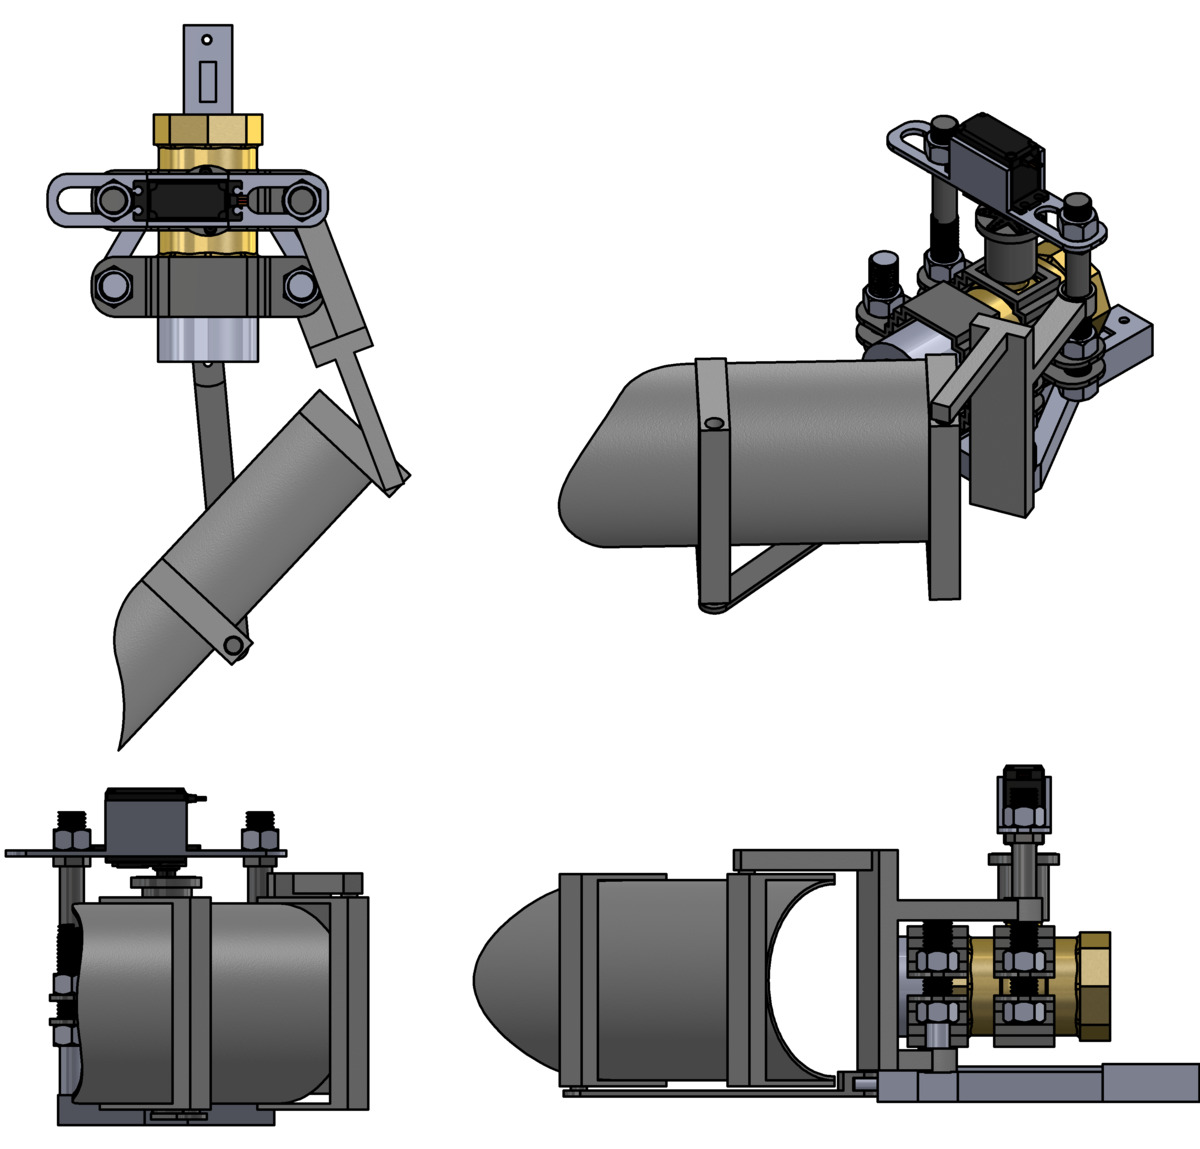
\includegraphics{Figures/DischargeFlowControlAssembly.PNG}
         \caption{Flow Diversion assembly}
         \label{fig:flow_diversion_assembly}
     \end{figure}
\par
Flow diversion assembly in conjunction with the flow control unit unit not only precisely controls the flow rate from the pipeline but also the discharge into the collecting tank or into the main reservoir. The linear motion of the actuator which is connected to the flap by mean of a rocker link achieves this function. A motion study simulation was conducted in SolidWorks. From  the study, in every step turn of the servo motor, the system effectively diverts the discharge to either into the collection tank or the main reservoir. 
\subsubsection{Discharge flow control Unit Assembly}
The assembly of the discharge flow control unit is shown in figure \ref{fig:unit_exploded_view}.
\begin{figure}[H]
    \centering
    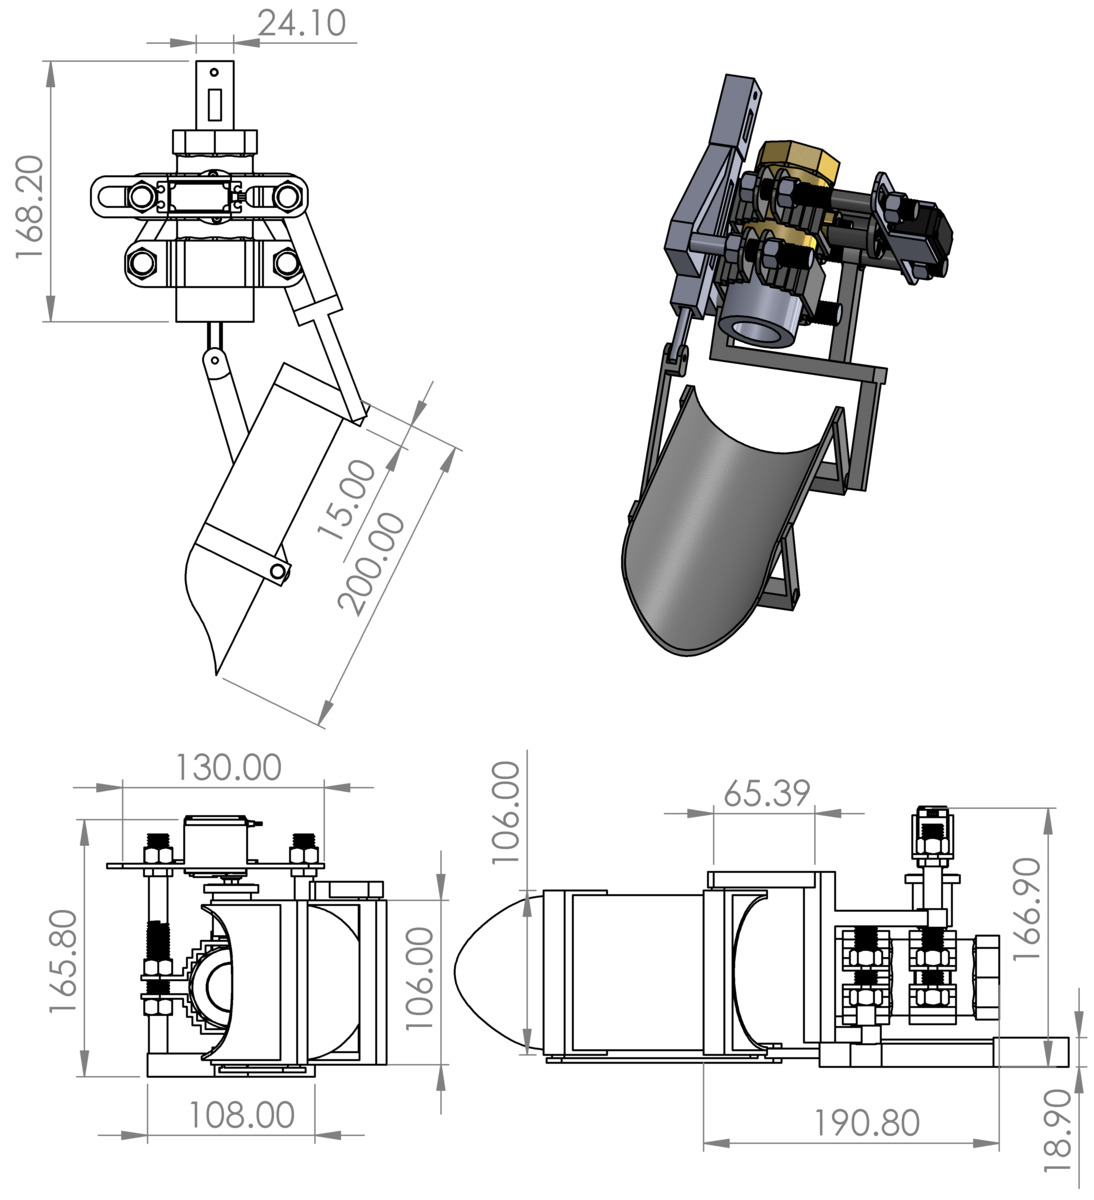
\includegraphics[width=\textwidth,height=0.75\textheight,keepaspectratio]{Figures/DischargeFlowControlAssemblyDrawing.PNG}
    \caption{2D Wireframe Model of the Final Assembly}
    \label{fig:final assembly}
\end {figure}
The exploded view of this unit is shown in figure \ref{fig:unit_exploded_view}.
\begin{figure}[H]
    \centering
    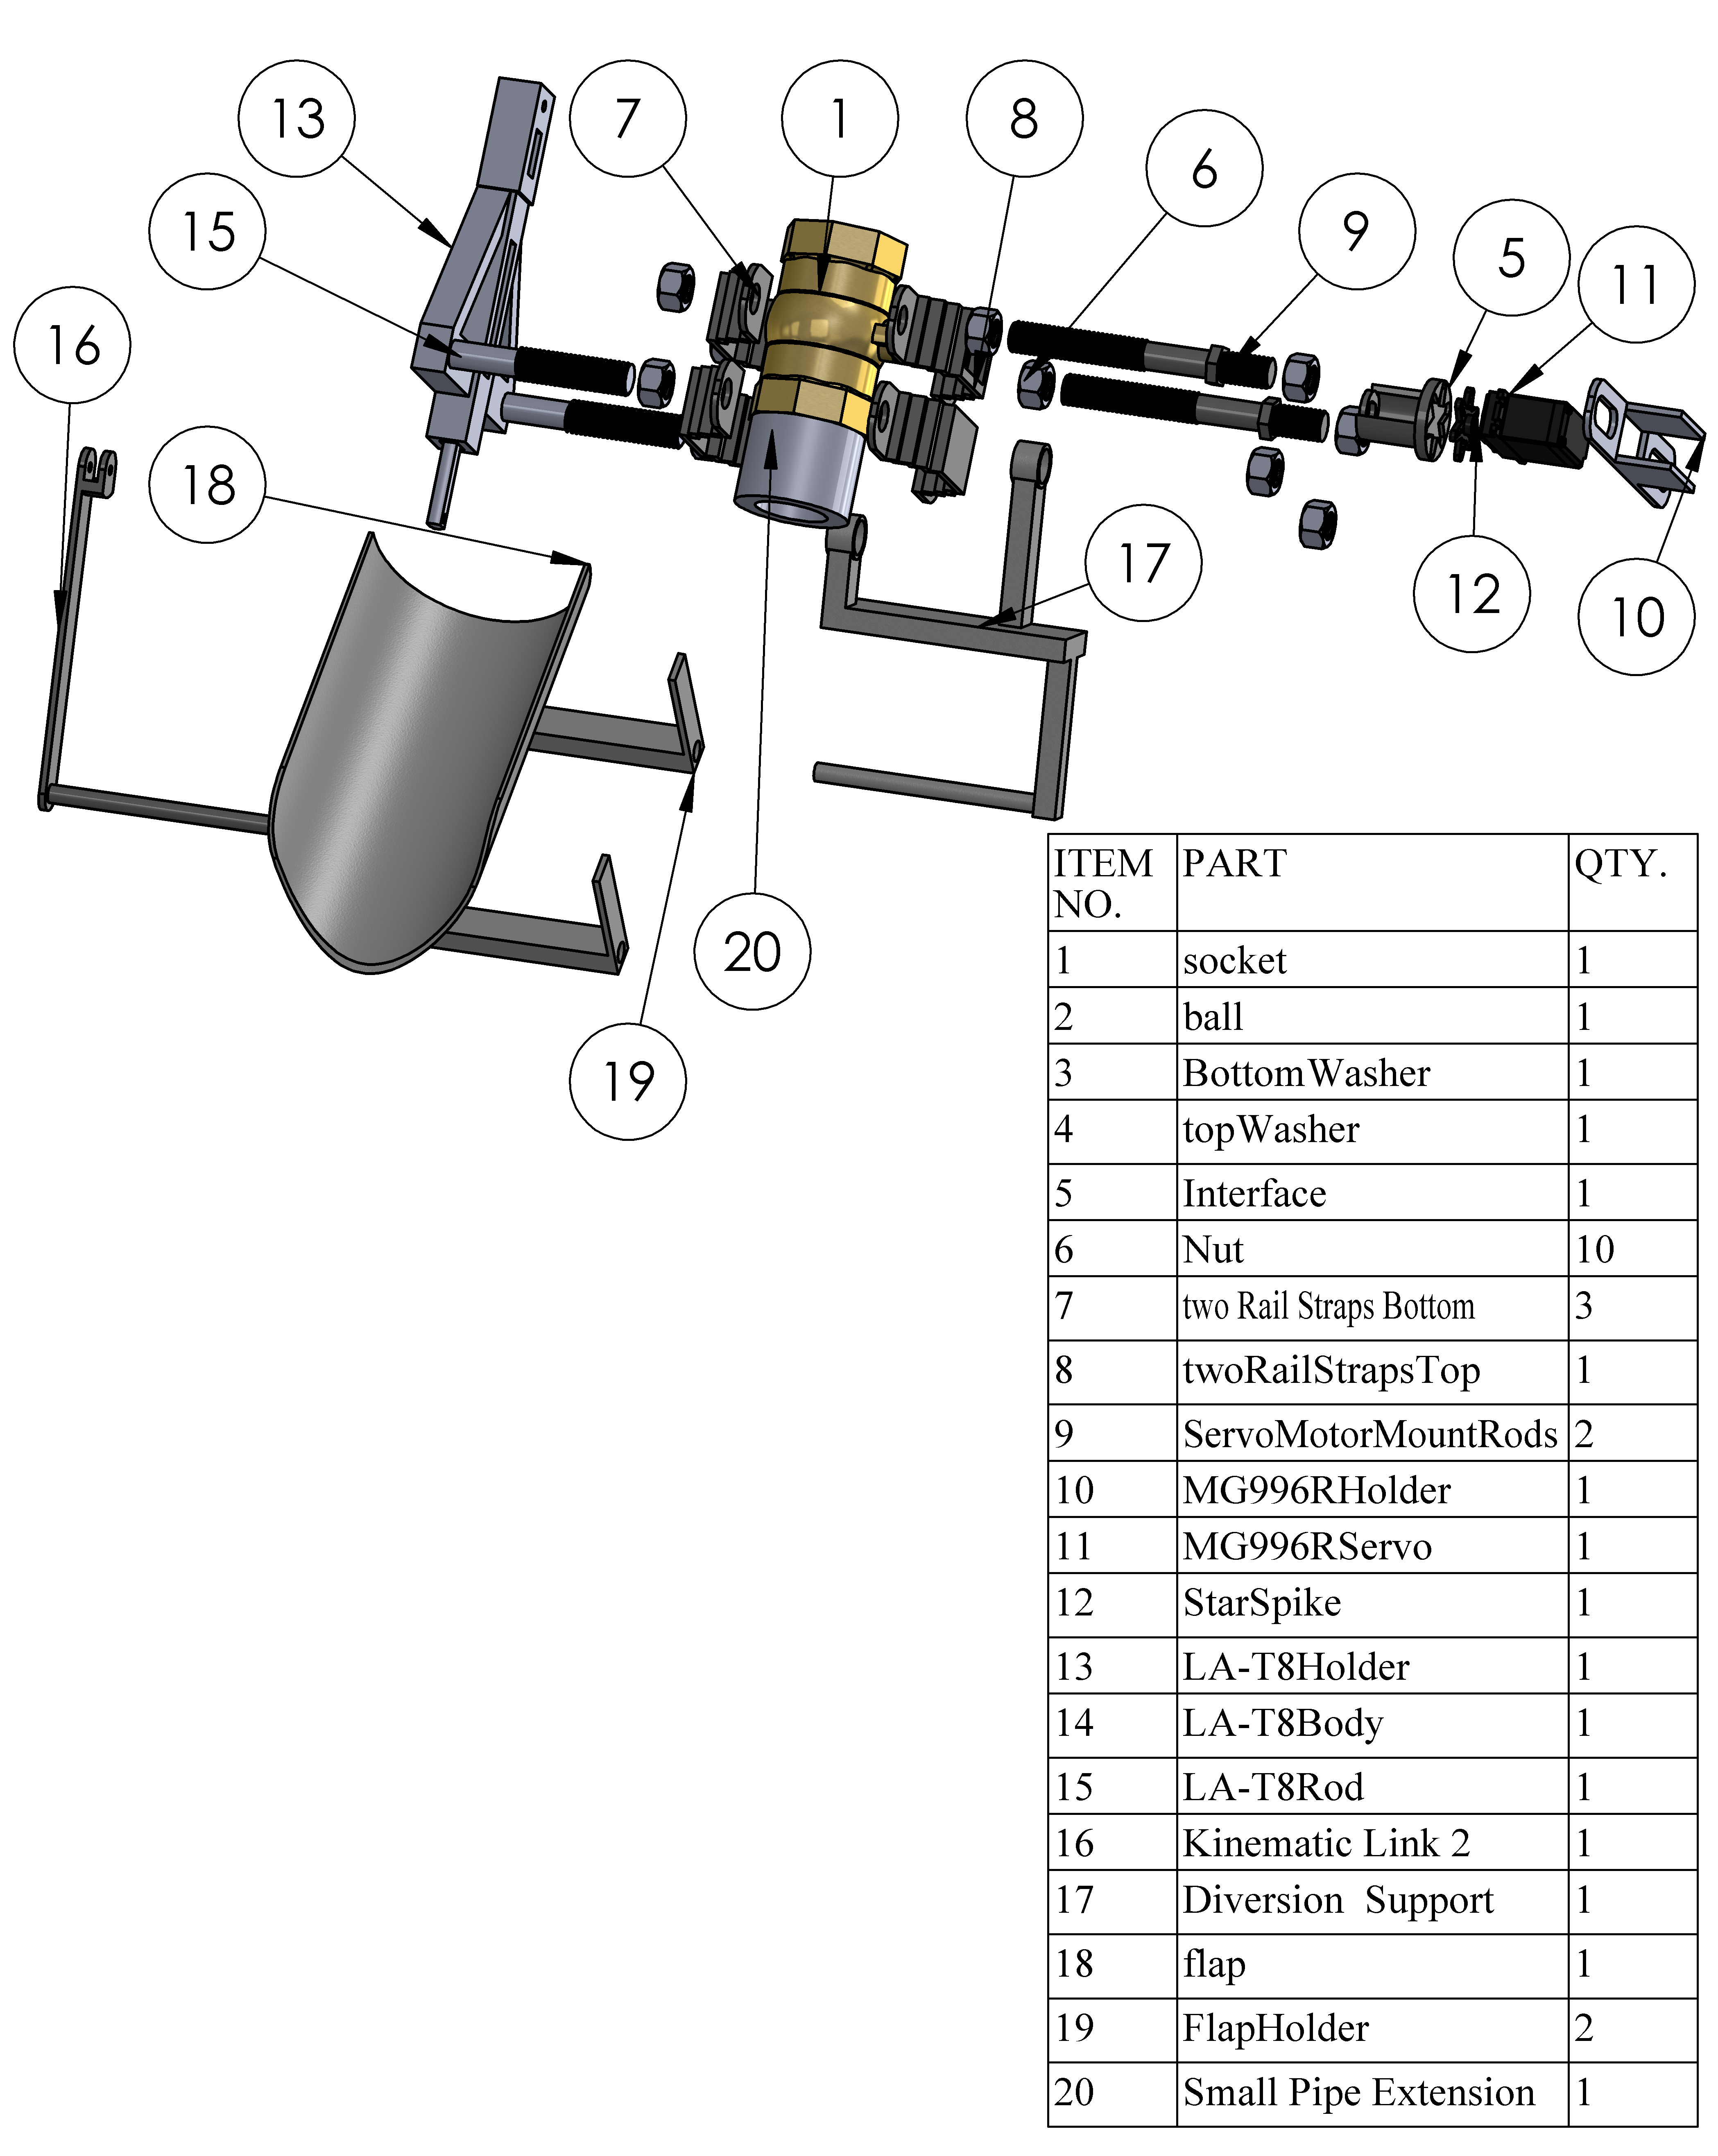
\includegraphics{Figures/DischargeFlowControlAssemblyExploded.PNG}
    \caption{Unit Exploded view}
    \label{fig:unit_exploded_view}
\end{figure}
From a motion study simulation in SolidWorks, the assembly appears to be able to regulate the fluid flow in steps as per the user's specifications. The diversion unit also seems to be able to divert the flow either to the main reservoir or to the discharge collection tank.

\subsection{Discharge Flow Handling unit}
\subsubsection{Discharge collection tank sub-unit}
The horizontal cylindrical tank selected for discharge collection process was subjected to a stress test of 1 Pascal. This was essential to determine the stress distribution in the whole tank tank system when fully filled with the discharge. This was essential in order to minimize the time taken to empty the tank. The results of the simulation is as shown in figure \ref{fig:tank_simulation_results}
  \begin{figure}[H]
         \centering
         \includegraphics[width=\textwidth, height=.4\textheight]{Figures/tank-Static-1-1-1.png}
         \caption{Tank simulation results}
         \label{fig:tank_simulation_results}
     \end{figure}
\par
From the simulation, the pressure in the tank was mostly concentrated at the sides close to the lower bottom line of the tank. The collected discharge will thus apply the same pressure on the tank and with the tap at the bottom, less time will be taken to empty the tank.
% \subsubsection{Outlet valve sub-unit}
% A solenoid valve was preferred to a butterfly valve because of its relatively cheaper price though the preferred size is slower.
% \subsubsection{Weight measurement sub-unit}
% Four load cells connected on a Wheatstone bridge were preferred to an ultrasonic approach to measure the weight of the collected discharge because the ultrasonic approach is unreliable.
% \subsubsection{Temperature measurement sub-unit}
% A DS18B20 immersible temperature sensor was selected for this subunit due to its reliability and sensitivity.
% \par
\subsubsection{Final assembly}
Figure \ref{fig:final assembly} shows the designed system attached to the Synthetic Hydro-Experimental Machine currently in use in JKUAT. The unit is designed as a plug-and-play plugin, in that it is not permanently fixed onto the machine but can  be removed. This is so as to ensure the machine can be used to perform other experiments.
\begin{figure}[H]
    \centering
    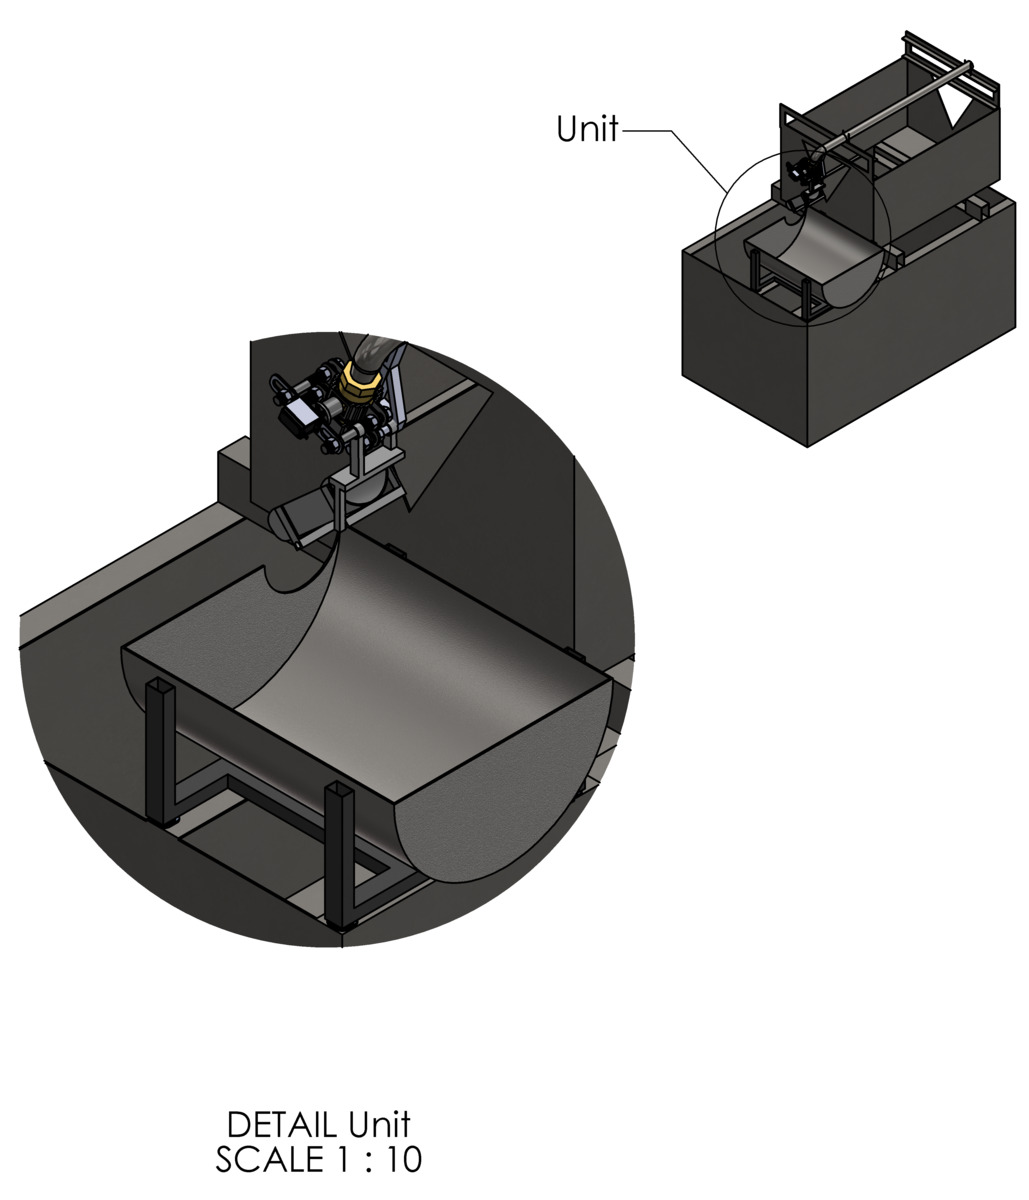
\includegraphics[width=\textwidth,height=0.75\textheight,keepaspectratio]{Figures/FinalAssemblyDetailed.PNG}
    \caption{Final Assembly with detailed view}
    \label{fig:final assembly}
\end{figure}
 The dimensions of the body are derived from the existing machine.
 \subsection{Full electrical circuit}
Figure \ref{fig:electrical_assembly} shows the electrical circuits of the two electronics: MG996R Servo motor and an LA-T8 Micro-linear actuator combined and simulated. The circuit uses a single external power supply from a 220V AC to 12V DC transformer. This is connected directly to the LA-T8 power circuit, and a regulator is used to step down the 12v to 6V for the MG996R stepper motor power circuit.
 \begin{figure}[H]
     \centering
     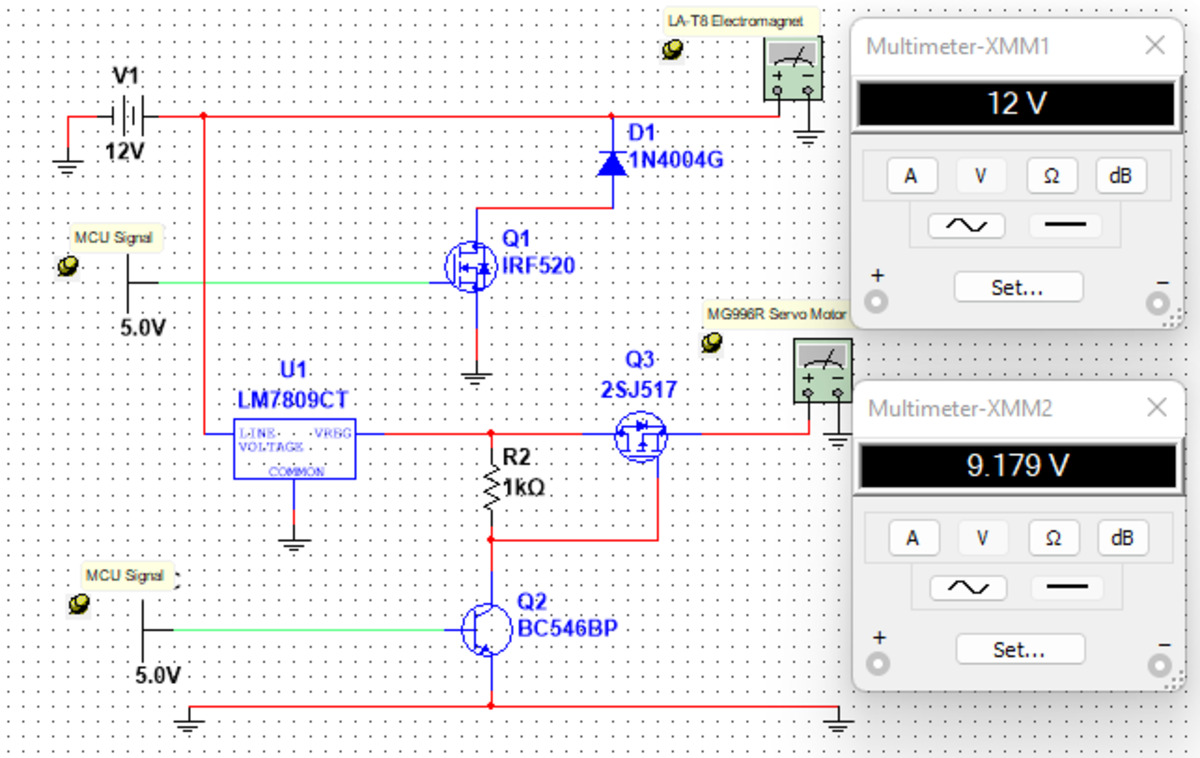
\includegraphics{Figures/FinalPartCircuit.png}
     \caption{Electrical assembly}
     \label{fig:electrical_assembly}
 \end{figure}

 
\subsection{Budget}
The table \ref{tab:budget} shows the budget of the project.
\begin{table}[H]
\centering
\caption{Budget}
\label{tab:budget}
\resizebox{\columnwidth}{!}{%
\begin{tabular}{|l|l|l|l|l|l|}
\hline
\textbf{Item No.} & \textbf{Item} & \textbf{Description} & \textbf{Unit Cost} & \textbf{No.} & \textbf{Total Cost} \\ \hline
1 & Servo Motor & MG996R(4.8Kg/cm) & 800 & 1 & 800 \\ \hline
2 & Linear Actuator & LA-T8 Linear Actuator & 3500 & 1 & 3500 \\ \hline
3 & Load cells & 50 Kg Load cells & 150 & 4 & 600 \\ \hline
4 & Load cell Amplifier & HX711 & 100 & 1 & 100 \\ \hline
5 & Temperature Sensor & DS18B20 Immersible & 300 & 1 & 300 \\ \hline
6 & Solenoid valve & 3/4''  Plastic & 900 & 1 & 900 \\ \hline
7 & MCU & STM32F407VET6 & 4400 & 1 & 4400 \\ \hline
8 & LCD & 320x240 Touch LCD & 1200 & 1 & 1200 \\ \hline
9 & Power MOSFET & IRF520 N-ch & 550 & 3 & 1650 \\ \hline
10 & Voltage Regulator & XL4015 DC-DC adjustable buck module & 400 & 3 & 1200 \\ \hline
11 & Transformer & AC 220V TO DC 12V 5A Transformer Power Supply & 1100 & 1 & 1100 \\ \hline
12 & Fabrication Cost & 3D printing \& Others & 10000 & 1 & 10000 \\ \hline
Total &  &  &  &  & \textbf{22600} \\ \hline
\end{tabular}%
}
\end{table}

    Some of the components such as LA-T8 micro-linear actuator, and the MCU with LCD,  are not available locally. The price indicated in the budget has their shipping cost included.
    Components such as strain-type load cells goes for Ksh. 250 a piece in Kenya. A temporary good deal was found on AliExpress, that reduced the price by half. The same case applied to the MCU board with the LCD. The fabrication cost indicated in the budget is the maximum possible estimate.


